\documentclass[a4paper]{article}

%% Language and font encodings
\usepackage[english]{babel}
\usepackage[utf8x]{inputenc}
\usepackage[T1]{fontenc}

%% Sets page size and margins
\usepackage[a4paper,top=3cm,bottom=2cm,left=3cm,right=3cm,marginparwidth=1.75cm]{geometry}

%% Useful packages
\usepackage{amsmath}
\usepackage{amssymb}
\usepackage{graphicx}
\usepackage[colorinlistoftodos]{todonotes}
\usepackage[colorlinks=true, allcolors=blue]{hyperref}
\usepackage{times}
\usepackage{url}
\usepackage{latexsym}
\usepackage{natbib}
\usepackage{graphicx}
\usepackage{paralist}
\usepackage{minted}
\graphicspath{ {figs/} }

%% \usepackage[numbers]{natbib}


\title{Multi-task Learning for Event-Participant Embeddings}
\author{Author: Xudong Hong \\ 
Supervisors: Asad Sayeed, Vera Demberg}


\begin{document}
\maketitle


\begin{abstract}
\noindent
We introduce several neural network models to learn embeddings containing both lexical and semantic features of events and event participants. Possible methods to compose word and semantic role representations are discussed. Making use of tensor factorisation on role-specific word embedding \citep{tilk2016event}, we represent the order-3 tensor with three matrices. Then we add non-linearity and construct the model as a neural network. The model is trained in multi-task style to perform both semantic role-filler prediction and semantic role prediction. Comparing to previous work, the model has improved on both semantic role/role-filler modelling and human thematic fit judgement correlations task. Moreover, the trained model has high accuracy on semantic role prediction. The high-level features of the model can be used in incremental semantic role labelling.  
\end{abstract}



\section{Introduction} \label{sec:intro}
In natural language understanding, the representation of events and their participants takes an important role. To understand different sentences, we need to focus on event-level information among them  (see Section \ref{sec:event}). For example, in sentences like: 
\begin{eqnarray}
    & &\text{The cook cut the cake with knife in the kitchen.}        \label{eg:sent1} \\   
    & &\text{In the kitchen, the cake is cut with knife by the cook.} \label{eg:sent2}
\end{eqnarray}
the event-level information is actually the same. The event is described by the predicate $cut$ and the participants of this event are $cook$, $cake$, $knife$ and $kitchen$. Although the syntactic roles of participant $cook$ in two sentences are different (subject in sentence \eqref{eg:sent1} and object in sentence \eqref{eg:sent2}), they are both the $cutter$ of the $cake$. This shared information can be capture by a level of shallow semantic representation: \textit{semantic roles} \citep{jurafsky2014speech}. 

Semantic roles express the abstract roles of a participant can take in an event. In this level of representation, event participants can be mapped to arguments where they located. Using \textit{thematic role}, an inventory of conceptual argument roles (see Section \ref{sec:semanticrole}), the two sentences in earlier example can be annotated as: 
\begin{eqnarray} \label{eg:thematic}
    \nonumber & &[_{\texttt{AGENT}} \text{The }\textbf{cook}]\ cut\ [_{\texttt{PATIENT}}\text{the }\textbf{cake}]\ [_{\texttt{INSTRUMENT}}\text{with }\textbf{knife}]\\  
    &   &[_{\texttt{LOCATION}}\text{in the }\textbf{kitchen}]. \\
    \nonumber & &[_{\texttt{LOCATION }}\text{In the }\textbf{kitchen}],\ [_{\texttt{PATIENT }}\text{the }\textbf{cake }]\ is \ cut\ \\
    &   &[_{\texttt{INSTRUMENT }}\text{with }\textbf{knife}]\ [_{\texttt{AGENT }}\text{by the }\textbf{cook}]. 
\end{eqnarray} 
where the event participants are actually head nouns or noun-noun compounds inside arguments of the predicate $cut$. $The\ cook$, volitional causer of the event, has a \texttt{AGENT} role. And $the\ cake$, the participant mostly affected by the event, has a \texttt{PATIENT} role. But it has been shown that it is hard to define thematic role formally. As a result, the PropBank \citep{palmer2005proposition} style semantic role model is introduced where each semantic role is associated with a specific verb sense. So the representation of two sentences can be unified as: 
\begin{equation*} \label{eg:probank}
\begin{aligned}
    & \text{Predicate: }&&cut.\textbf{01} \\
    & \text{Arguments: }&&[_{\texttt{ARG0 }}\text{The }\textbf{cook}], \ [_{\texttt{ARG1 }}\text{the }\textbf{cake}], \ [_{\texttt{ARGM-MNR }}\text{with a }\textbf{knife}], \\
    &                   &&[_{\texttt{ARGM-LOC }}\text{in the }\textbf{kitchen}]
\end{aligned}
\end{equation*} 
where each argument is assigned with a semantic role label. $cut.01$ is the verbal predicate $cut$ with sense $01$ which is \textit{"make an incision or separation"}. Now the \texttt{ARG0} role can be defined exactly as \textit{"the subject which makes incision"}. To obtain this representation from raw text, one needs to solve semantic role labelling task (see Section \ref{sec:srl}). 

Since both raw words and semantic role labels are symbols, it has limited representing power. If someone wants to compare events quantitatively, it is not possible to use the \textit{symbolic representation} where each symbol represents a single state of the entry. There are some previous works construct numerical representation of linguistic units e.g. \textit{Distributional semantic model} (DSM) (see Section \ref{sec:dsm}). Among them, \textit{Distributed representation} of words, also named as \textit{word embedding}, is a well-established technique based on continuous feature space. Each word is represented by a low-dimensional dense vector with real number parameters which are learnt during training of a prediction task given the context. There are many efforts on learning word embeddings from large-scale corpora (see Section \ref{sec:repr}). 


\begin{table}[t]
\centering
\begin{tabular}{l|ll}
\textbf{Event 1}    &   \textbf{Event 2}    &   \textbf{Similarity} \\
                    &   \textbf{Foil Event} &   \textbf{Similarity} \\  \hline
(investor, buy, share)      &   (investor, purchase, share)     &   0.96    \\
                            &   (share, purchase, investor)     &   0.81    \\    \hline
(employee, buy, property)   &   (employee, purchase, property)  &   0.95    \\
                            &   (property, purchase, employee)  &   0.80    \\    \hline
(supporter, buy, ticket)    &   (supporter, purchase, ticket)   &   0.96    \\
                            &   (ticket, purchase, supporter)   &   0.83    \\
\end{tabular}
\caption{\label{tab:eventsim} Some examples of similarity scores between two events using event embedding vectors in NNRF model. The metric is cosine similarity. }
\end{table}

\subsection{Main Problem and Previous Work}
The main problem is that only a few works learn embeddings at the level of events. \citet{tilk2016event} proposed two models to learn a representation of events and their participants. To obtain a probability distribution over \textit{role-fillers} given event information, the models aim to perform \textit{role-filler prediction}: 
\begin{itemize}
    \item  In each event, given the role label of one target word, and also given all other words and their role labels, the task is to predict the target word to fill the target role,
\end{itemize}
where the verbal predicate is considered as a special role $verb$ which is not in PropBank style semantic roles. The representation, named as \textit{role-specific word embedding}, learnt by those models is organised into an order-3 tensor. This means that for each word and each role, there is an embedding vector. To reduce the number of parameters, they factored the tensor into three matrices. They reported great improvement over previous systems on thematic fit evaluation and competitive performance on event similarity evaluation. 

However, there are some limitations in their work. Firstly, the definition of the notion \textit{role} is vague. It is hard to explain why predicates and semantic arguments are treated as the same, though they have a special role $verb$ for verbal predicates. This leads to an ambiguous definition of \textit{role-filler} which originally means the argument to fill one specific semantic role. Their representation is also inconsistent with event representation in first-order logic. 
% * <asayeed@mbl.ca> 2017-11-13T22:29:40.729Z:
% 
% Well I don't know if they're "major" disadvantages :)
% 
% ^ <xhong@coli.uni-saarland.de> 2017-11-16T12:58:14.475Z:
% 
% Could you please give a more specific comment? Do you mean that I should change it to ‘limitation'? 
% 
% ^ <asayeed@mbl.ca> 2017-11-16T21:52:11.087Z:
% 
% Yes, that is a better word.
%
% ^ <xhong@coli.uni-saarland.de> 2017-11-17T15:10:36.118Z.

In addition to that, there is a problem of event embedding similarity if we only focus on role-filler prediction. Because of the smoothing effect of distributed representation, the event embeddings with same argument words but different roles can be very similar to each other. For example, considering a original event $([_{\texttt{ARG0}} \text{investor}], buy, [_{\texttt{ARG1}}\text{share}])$ and the foil event $([_{\texttt{ARG0}}\text{share}], purchase, [_{\texttt{ARG1}}\text{investor}])$, the model shows high similarity score between them. The foil event is unlikely to happen in real world, so human will have a lower similarity judgement score between it and the original event. But for the similar event $([_{\texttt{ARG0}}\text{investor}], purchase, [_{\texttt{ARG1}}\text{share}])$ and the original event, human will have a high similarity judgement score. So the NNRF model is incompatible with human cognition. More examples are shown in Table \ref{tab:eventsim}. 
% * <asayeed@mbl.ca> 2017-11-13T22:30:35.273Z:
% 
% "based" event? ("foil" is pretty clear)
% 
% ^ <xhong@coli.uni-saarland.de> 2017-11-16T12:54:58.718Z:
% 
% Changed to 'original event'
%
% ^.

Furthermore, the factored order-3 tensor structure is not fully explained. Along with the rapid growth of architecture complexity, explainability of models is becoming more and more important. Yet they did not give a thorough explanation of the word embedding they obtained. Moreover, there is no evaluation of their word embedding. As a result, it is risky to use the embedding on other tasks. 

Last but not least, although the tensor-like structure of embedding is efficient and flexible, the training of the models are burdened by the gradient explosion or vanishing problem. Because in a factored order-3 tensor, each parameter is represented by a product of three parameters. To tackle this problem from the training aspect, they used Adagrad \citep{duchi2011adaptive} which adjusts learning rate during training. Although it alleviated the problem, it is not a solution on model architecture aspect. 


\subsection{Major Tasks}
In this paper, we present several multi-task neural network models to learn embeddings at the inner level of an event. With a view to the explainability of the task, we separate \textit{role-filler prediction} into two sub-tasks: 
\begin{itemize}
  \item  \textbf{Participant prediction}: in each event, given the predicate, the semantic role label of one target participant, the other participants and their semantic role labels, the task is to predict the target participant to fill the semantic role. 
  \item  \textbf{Predicate prediction}: in each event, given all participants and their semantic role labels, the task is to predict the predicate. 
\end{itemize}
Since lexical features of participant and predicate are homogeneous, we can consider each of them as a word. To get rid of ambiguity, we define \textbf{semantic role labels} as a set which contains semantic role labels in PropBank style for event participants and a special semantic role label for predicates. In order to tackle the similarity problem in event embedding stated above, we add one more auxiliary task which is: 
\begin{itemize}
  \item  \textbf{Semantic role prediction}: in each event, given one target word, and all other words and their semantic role labels, the task is to predict the target semantic role label. 
\end{itemize}
By forcing the models to solve semantic role prediction during training, the event embeddings with same words but different roles will be distinguished. 

\subsection{Model Design and Experiments}
Inspired by the role-specific word embedding, we define the \textbf{event-participant embedding} formally as the joint embedding of predicates that denote events and participants of events. The embedding vectors are stacked together to construct an order-3 tensor where each vector is indexed by a 2-tuple $(word, role\ label)$. As a result, each word can be represented as a matrix, indexed by a 1-tuple $(word)$, which can be considered as word embedding (see Section \ref{sec:epe}). Although the event-participant embedding is a versatile representation, it suffers curse of dimensionality. So we apply tensor factorisation on the event-participant embedding tensor, which represents the tensor with three matrices. After detailed analysis in the tensor space, we demonstrate that these matrices can be interpreted as word embedding, semantic role label embedding and weight of linear mapping correspondingly (see Section \ref{sec:tf}). 

Using the same event-participant embedding as input, we add non-linearity to the models to construct multi-task neural networks. To perform both role-filler prediction and semantic role prediction, we design two classifiers with their own loss functions. The models are optimised with different weight of each task (see Section \ref{sec:mtrf}). We find that tuning the loss weight results in models having their own advantages in different aspects. When it comes to the construction of event representation, there are two cases: participant order is known or unknown. In order to build a model which is compatible with first-order logic representation where conjunction connective does not imply order, we focus on the case that participant order is not given. After comparing several composition methods, we present an effective method to compose the event-level embedding using features from the hidden layer (see Section \ref{sec:bop}). It has been shown that gradient exploding or vanishing problem is more serious in training model with factorised tensors \citep{sutskever2011generating}.  Making use of the idea in residual learning, we add one skip connection inside the factor tensor (see Section \ref{sec:residual}). We find that this method can help with learning a better event-participant embedding.

To compare with previous baselines, all models are trained, validated and tested on the same large scale corpus. We tune hyper-parameters to optimise for different purposes (see Section \ref{sec:exp}). On both three tasks, we compute the perplexity for each model(see Section \ref{sec:wordprediction}, \ref{sec:roleprediction}). The output probabilities of the models on word prediction are evaluated on human thematic fit judgement correlation task (see Section \ref{sec:thematicfit}). The word embeddings are evaluated on several word similarity tasks (see Section \ref{sec:wordsim}). Last but not least, the event embeddings are evaluated on an event similarity correlation task (see Section \ref{sec:eventsim}). The results show that our models have significant improvement over the current best system on specific evaluations while has state-of-the-art performance on the other evaluations. The word embedding and event embedding extracted from the event-participant embedding we learnt also has state-of-the-art performance. 
% * <asayeed@mbl.ca> 2017-11-13T22:34:00.165Z:
% 
% This is a very thorough high-level overview, but it's easy to get lost.  Maybe put in some subsections or bullet points?
% 
% ^ <xhong@coli.uni-saarland.de> 2017-11-16T12:59:10.662Z:
% 
% Is it only the paragraph above the comment or all three about contribution? 
%
% ^ <asayeed@mbl.ca> 2017-11-16T21:53:28.466Z:
% 
% There are parts of the above three paragraphs that look like "steps" and some that read like "reasons".  I think they could be reorganized so that we can follow all the moving parts.  So yeah, all three.
%
% ^.

\subsection{Contribution}
Our model is a state-of-the-art system of thematic fit correlation task. The selectional preference features are useful for referent prediction in discourse-level \citep{modi2017modeling}. In simultaneous machine translation between language pairs with different verb position, adding predicate prediction leads to better translations \citep{grissom2014don}. The word embedding we learn can be further employed in discourse relation classification \citep{shi2017need, rutherford2017systematic}, paraphrase detection, word sense disambiguation, sentiment analysis and machine translation. The composite embedding of predicate and target head word can be used for argument classification in semantic role labelling \citep{roth2016neural}. Further, this model can be employed in incremental semantic parsing \citep{konstas2014incremental, konstas2015semantic} or inferences of logical forms (TODO: add ref). 



\newpage
\section{Background}


\begin{table}[t]
\centering
\begin{tabular}{l|l}
\textbf{Thematic Role}  &   \textbf{Definition} \\ \hline
AGENT                   &   The volitional causer of an event \\
PATIENT (THEME)         &   The participant most directly affected by an event \\
INSTRUMENT              &   The inanimate force or object used in an event \\
LOCATION                &   The location or spatial orientation of the event \\
\end{tabular}
\caption{\label{tab:thematic} Definitions of common thematic roles.}
\end{table}


\subsection{Event Knowledge and Event Representation} \label{sec:event}
In psycholinguistics and cognitive science, experiments have shown that event knowledge plays a crucial role in human sentence processing \citep{camblin2007interplay}. On one hand, predicates prime event participant referring to good fillers of their semantic role in an event \citep{ferretti2001integrating}. On the other hand, priming effect can be also found from event participants to predicates \citep{mcrae2005basis}. These two works reveal that model performances of predicate prediction and participant prediction can be evaluated via correlation with human judgement. In a wider range, event-level information affects verbal arguments processing of human \citep{bicknell2010effects}. Comprehenders integrate information not only from predicate but also other event participants mentioned in discourse. Although there are plenty of results from different forms of psycholinguistic experiments like event-related potential, eye-tracking and human judgement, most of these experiments have a relatively small size of evaluation entries and a limited number of participants. It has been shown that corpus-based method can be considered as a large-scale simulation of human acquisition of linguistic or conceptual information from the world \citep{landauer1997solution}. To verify the results from psycholinguistic experiments, it is necessary to build corpus-based cognitive models of events. 

In early research, events were represented using first order logic. For the event in the example sentence (\ref{eg:sent1}), the representation is:
\begin{equation*} \label{eg:fol}
\begin{aligned}
    & cut(\text{cook}, \text{cake}) \land with(\text{knife}) \land in(\text{kitchen}) \\
\end{aligned}
\end{equation*}
where it is hard to refer to predicates. Later on, \citet{davidson1967logical} proposed a method that linguistic predicates consider an event as one of their logical arguments explicitly. So the representation of the sentence (\ref{eg:sent1}) becomes: 
\begin{equation*} \label{eg:davidsonian}
\begin{aligned}
    & \exists e\ cut(e, \text{cook}, \text{cake}) \land with(e, \text{knife}) \land in(e, \text{kitchen}) \\
\end{aligned}
\end{equation*}
where the predicate $cut$ is a description of an event $e$. This representation, named as \textit{Davidsonian event representation}, has a drawback that it is hard to distinguish the roles of $cook$ and $cake$. Combining with thematic roles mentioned in session \ref{sec:intro}, \citet{parsons1990events} updated the representation to: 
\begin{equation} \label{eg:neodavidsonian}
\begin{aligned}
    \exists e\ cut(e)
    & \land \text{AGENT}(e, \text{cook}) \land \text{PATIENT}(e, \text{cake}) \\
    & \land \text{INSTRUMENT}(e, \text{knife}) \land \text{LOCATION}(e, \text{kitchen}) \\
\end{aligned}
\end{equation}
where each thematic role is acting as a logical predicate of the event $e$ and the corresponding participant. This representation, named as \textit{neo-Davidsonian event representation}, is highly compatible with semantic role models. 
% * <asayeed@mbl.ca> 2017-11-13T22:37:07.932Z:
% 
% Unfortunately neo-Davidsonian representations and the psycholinguistic work on this topic are only loosely connected. We introduced neo-Davidsonian representations to allow for incrementality in PLTAG-based semantic parsing.  Otherwise, most psycholinguistic work doesn't care about the formal status of the event.  Unless you want to justify things in terms of the output representation of a parse, is this necessary?
% 
% ^.


\subsection{Semantic Role Model} \label{sec:semanticrole}
Thematic role is the oldest semantic role model which is formalised by \citet{gruber1965studies} and \citet{fillmore1968case} in modern time. The inventory of roles usually contains AGENT, PATIENT, INSTRUMENT and LOCATION \citep{aarts2013english}. Table \ref{tab:thematic} shows informal definitions of them \citep{jurafsky2014speech}. One disadvantage of thematic roles is that the range of role inventory is difficult to decide. Even worse, the formal definitions of thematic roles are controversial. 

The Proposition Bank (PropBank) is an annotated corpus of semantic roles based on Penn TreeBank \citep{palmer2005proposition}. It also provides an effective semantic role model which we will adopt. Table \ref{tab:propbank} shows definitions of semantic roles in PropBank style used in this paper. The definitions are based on the PropBank Annotation Guidelines \citep{bonial2010propbank}. Arguments required for the valency of a predicate are listed with numbers. Modifiers, which are relatively stable across predicates, are marked with ArgMs. While PropBank focuses on verbal predicates, NomBank adds annotations to nominal predicates \citep{meyers2004nombank}. 


\begin{table}[t]
\centering
\begin{tabular}{l|l} 
\hline
\textbf{PropBank Semantic Role}  &   \textbf{Definition} \\ \hline
Arg0                    &   proto-agent, the argument that most likely to be the agent, \\ 
                        &   volitional causer or experiencer \\ \hline
Arg1                    &   proto-patient, the argument that most likely to be the patient \\ \hline
Arg2                    &   the instrument, benefactive or attribute \\ \hline
Arg3                    &   the starting point, benefactive or attribute \\ \hline
Arg4                    &   the ending point \\ \hline
ArgM-LOC                &   the argument that indicates where the action takes place \\ \hline
ArgM-MNR                &   the argument that specifies how the action is performed \\ \hline
ArgM-TMP                &   the argument that shows when an action took place \\ \hline
ArgM-PNC                &   the argument that shows motivation for some action \\ \hline
ArgM-CAU                &   the argument that indicates the reason for an action \\ \hline
\end{tabular}
\caption{\label{tab:propbank} Examples of semantic roles in PropBank style.}
\end{table}
% * <asayeed@mbl.ca> 2017-11-13T22:39:14.487Z:
% 
% There are even more, but we don't use them.  And we don't use ARGM-CAU, do we?
% 
% ^ <xhong@coli.uni-saarland.de> 2017-11-16T13:00:01.637Z:
% 
% This is a summary of PropBank role. The role labels we use are in section 3. 
% 
% ^ <asayeed@mbl.ca> 2017-11-16T21:54:38.832Z:
% 
% OK make it clear that this is only a sample of the ARGM ones.
%
% ^ <xhong@coli.uni-saarland.de> 2017-11-17T15:40:07.201Z.


\subsection{Semantic Role Labelling} \label{sec:srl}
The \textit{semantic role labelling} (SRL) task is to assign semantic role labels to arguments of predicates in sentences automatically. It is a well-study task which was defined formally at CoNLL 2004, 2005 shared tasks which aimed to annotate phrasal arguments of verbal predicates in the sentences \citep{carreras-marquez:2004:CONLL, carreras-marquez:2005:CoNLL}. The CoNLL 2008, 2009 shared tasks introduced a new task where the semantic dependencies are annotated instead of phrasal arguments \citep{surdeanu-EtAl:2008:CONLL, hajivc-EtAl:2009:CoNLL-2009-ST}. 

After many years of research, pre-trained semantic role labelling systems are quite reliable. Generally speaking, modern SRL system is a statistical model that can predict the semantic role labels given the sentences. Many early work used syntactic parses as input and estimate classifiers locally with a set of constraints \citep{punyakanok2008importance}. \citet{tackstrom2015efficient} interpreted the model as a graphical model and use a multi-layer neural network to enforce the constraints. Other works focus on the application of distributed representation to avoid feature engineering and result in better generalisation. \citet{collobert2007fast, collobert2011natural} proposed a convolution neural network model using a distributed representation that only relies on lexical features. The fine-tuned model with additional features, SENNA, has competitive performance. The running time of SENNA is fast so it can be used on a large corpus. 
% * <asayeed@mbl.ca> 2017-11-13T22:40:52.091Z:
% 
% SENNA isn't state of the art performance anymore, is it? And after citing Täckström 2015, you can't say that 2007 and 2011 papers are "later works", now can you?
% 
% ^ <xhong@coli.uni-saarland.de> 2017-11-16T13:03:41.920Z:
% 
% Changed to 'Other works'
%
% ^.


More recently, \citet{lei-EtAl:2015:NAACL-HLT} employ low-rank tensor factorisation to induce a compact representation of the full cross product of atomic features. \citet{roth2016neural} proposed PathLSTM which made use of dependency path as input. \citet{marcheggiani2017simple} claimed that syntactic features are not necessary for semantic role labelling and proposed a deep LSTM model to obtain competitive performance. 

However, most of these works only assign labels to whole constituents instead of syntactic heads that are denoting event participants. \citet{SayeedEtAl2015} proposed an unsupervised method of assigning semantic roles to syntactic heads in arguments. The semantic role labels are extracted using SENNA. Then the head nouns are extracted from arguments using Malt Parser, a state-of-the-art dependency parser \citep{nivre2006maltparser}, together with hand-crafted heuristics. The annotated corpus they constructed is named as \textbf{RW-eng}. 


\subsection{Distributional Semantic Model} \label{sec:dsm}
Distributional semantic model (DSM) is a corpus-based method to construct numerical semantic representation. DSM depends on \textit{distributional hypothesis} \citep{harris1954distributional, miller1991contextual} claiming that the semantic similarity between two linguistic units can be measured by the overlap among their contexts. A DSM can be viewed as an order-2 tensor where one dimension is indices of words (or lexical units) and another dimension is features that used to capture context information. Generally, in early work of DSM, a matrix was constructed based on lexical co-occurrences of words in a large corpus. Then each word can be represented by a high-dimensional sparse vector in this matrix. The semantic similarity between two units can be quantified as the similarity of two representation vectors. This, however, does not consider the linguistic information within the context. To include such information, later work encode syntactic relation or lexico-syntactic pattern \citep{pado2007integration, erk2008structured, rothenhausler2009unsupervised} (TODO: performance?). 

\citet{baroni2010distributional} claimed that it is possible to construct a general model for semantic memory, a stable long-term knowledge of human, to tackle different semantic tasks. They proposed \textit{Distributional Memory} (DM) framework which is an order-3 tensor which contains word-relation-word tuple. Performing matricisation on the tensor onto a matrix, vectors from different semantic spaces can be obtained. On tasks of a broad range, their best model, named as TypeDM, obtained competitive performance. This can be interpreted as the advantage of the distributional representation on multiple semantic tasks. Furthermore, the tensor like structure is both flexible and expressive for semantic information modelling. 

In addition to syntactic information, \citet{sayeed2014combining} extracts shallow semantic representation using semantic role labeller SENNA and constructs DM upon them. Combining syntactic and semantic features, they build a fully unsupervised distributional memory model, named as SDDM, especially for thematic fit judgement task. SDDM outperforms syntax-based thematic fit model by a large margin, which indicates that semantic information is essential in the thematic fit task. 

There are three major drawbacks of the distributional semantic model. Firstly when it comes to practice, the semantic space of DSM is high-dimensional and sparse. When someone wants to induce on complex events with a large number of participants, the size of representation becomes enormous. It is time or space consuming to use this kind of representation in practice. In addition, the parameters of the vectors are discrete in count-based vector space. Although many alternative weighting functions and smoothing techniques have been proposed, it is hard to decide which is the most optimised. Last but not least, these models usually suffer the curse of dimensionality. Because the Euclidean distance between two vectors is meaningless in high-dimensional space, when the representation vectors are used as input of distance-based algorithms like nearest-neighbour classifier or clustering, the result can be unexpected. Thus we need a better representation model in this paper. 
% * <asayeed@mbl.ca> 2017-11-13T22:43:00.518Z:
% 
% Why is using sparse vectors infeasible for complex events? Because of the multiplicative nature of event composition in e.g. the Lenci 2011 (?) model of compositionality via DMs.
% 
% ^ <xhong@coli.uni-saarland.de> 2017-11-16T13:10:12.720Z:
% 
% I added more details. It is changed to ' the size of representation becomes enormous. It is time or space consuming to use this kind of representation in practice. '
% 
% ^.


\subsection{Distributed Representation} \label{sec:repr}
Distributed representation, pioneered by \citet{hinton1986learning}, is an effective method to handle sparsity and curse of dimensionality in symbolic representation. In general symbolic representation like \textit{one-hot representation}, where one binary value is $1$ and the others are $0$ in representation vectors, the binary values are mutual exclusive. If each representation vector has $n$ features, it can only represent $n$ different states of the entry. In distributed representation, $n$ feature with $k$ possible values can describe $k^n$ different states \citep{Goodfellow-et-al-2016}. This is why distributed representation is powerful. 

The distributed representation of words, popularly known as word embedding, can be learnt in the training of \textit{neural net language model} \citep{bengio2003neural}. Most of the early works aimed to solve language modelling which is the task to predict the target word given its context. Unlike DSMs or other count-based semantic models, the parameters in distributed representation vectors are learnt during the training of neural net language models. Later these models were further improved by making use of sequential information in the previous context of target words. This can be done by adding recurrent units to hidden layers of neural net language model \citep{mikolov2010recurrent}. To learn high quality word embeddings with million words in the vocabulary from a billion scale of text, \citet{mikolov2013efficient} proposed two models, \textit{CBOW} and \textit{Skip-gram}, based on logistic regression. Context is the words around the target word in both models. In CBOW model, context representation is the sum of word embedding vectors of the words in the context. In Skip-gram model, the target word is used to predict the words in the context. The system they built, famously known as \textit{word2vec}, obtained competitive performance against more complex neural networks on syntactic and semantic relation tasks. To tackle multiple tasks in natural language processing, \citet{collobert2011natural} proposed a model which shares the word embedding across tasks of language modelling, part-of-speech tagging, chunking, named entity recognition, semantic role labelling. 



\newpage
\section{Representation of Predicates and Participants}
We intend to learn meaningful representation of event structure in semantic space. In \textit{neo-Davidsonian event representation}, we notice that linguistic predicates can be further generalised. So we define a special role PRD for predicates. The example \ref{eg:neodavidsonian} can be rewritten as: 
\begin{equation*} \label{eg:symbolic-thematic}
\begin{aligned}
    \exists e\ \text{PRD}(e, \text{cut})
    & \land \text{AGENT}(e, \text{cook}) \land \text{PATIENT}(e, \text{cake}) \\
    & \land \text{INSTRUMENT}(e, \text{knife}) \land \text{LOCATION}(e, \text{kitchen}) \\
\end{aligned}
\end{equation*}

If we specify the sense of the predicate $cut$, thematic roles can be replaced with PropBank style semantic roles as: 
\begin{equation*} \label{eg:symbolic-semantic}
\begin{aligned}
    \exists e\ \text{PRD}(e, \text{cut.01})
    & \land \text{ARG0}(e, \text{cook}) \land \text{ARG1}(e, \text{cake}) \\
    & \land \text{ARGM-MNR}(e, \text{knife}) \land \text{ARGM-LOC}(e, \text{kitchen}) \\
\end{aligned}
\end{equation*}
This is a representation of the event in first order logic. We define a semantic role model for this paper. We join PropBank semantic roles and the special role PRD together as semantic roles. So the semantic role labels we use in this paper are defined in Table \ref{tab:semantic}. As we mention above, semantic arguments can be represented by the syntactic head words, so the notion of \textit{argument} in PropBank role labels is replaced by \textit{event participant}. 

% * <asayeed@mbl.ca> 2017-11-13T22:45:29.318Z:
% 
% Again do we need to commit to this kind of representation here?  I'm not saying categorically not to do it, merely that it needs to be justified.
% 
% ^.

\begin{table}[t]
\centering
\begin{tabular}{l|l|l} 
\hline
\textbf{ID} &   \textbf{Semantic Role Label}    &   \textbf{Definition} \\  \hline
0           & PRD       &   the predicate denoting the event \\ \hline
1           & ARG0      &   proto-agent, the event participant that most likely to be the agent, \\     &&   volitional causer or experiencer \\ \hline
2           & ARG1      &   proto-patient, the event participant that most likely to be the patient, \\ &&   the event participant which is being affected by the action \\ \hline
3           & ARG2      &   the event participant which is secondly likely to be the patient,  \\       &&   the benefactive or attribute \\ \hline
4           & ARGM-MNR  &   the event participant that specifies how the action is performed \\ \hline
5           & ARGM-LOC  &   the event participant that indicates where the action takes place \\ \hline
6           & ARGM-TMP  &   the event participant that shows when an action took place \\ \hline
\end{tabular}
\caption{\label{tab:semantic} Definitions of semantic role labels in this paper.}
\end{table}


\subsection{Event-Participant Embedding} \label{sec:epe}
After obtaining the semantic role model, we define the symbolic representation for words. Word $a_i$ is encoded as one-hot row vector $\mathbf{w}_i$ where $|\mathbf{w}_i| = |V|$ and $V$ is the word vocabulary. In this vector space, words are mutual exclusive to each other. Similarly, we can represent semantic role label $b_j$ using one-hot encoded column vector $\mathbf{r}_j$ where $|\mathbf{r}_j| = |R|$ and $R$ is the set of semantic role labels. 

Further, we need to obtain a distributed representation that is continuous in the feature space. So we compute the inner product between $\mathbf{w}_i$ and a embedding matrix $\mathbf{A} \in \mathbb{R}^{|V| \times d}$ as $\mathbf{A}_{(i)} = \mathbf{w}_i \mathbf{A}$. The vector $\mathbf{w}_i$ is now mapped to low-dimensional vector $\mathbf{A}_{(i)} \in \mathbb{R}^d$ which is the $i$-th row of matrix $\mathbf{A}$. The symbolic representation of words is transformed into word embedding. 

In addition to word embedding, we want to learn the representation of words given a specific semantic role label. We add one more dimension of semantic role label to the word embedding matrix and obtain a third-order tensor $\mathbf{T} \in \mathbb{R}^{|V| \times |R| \times d}$. For each word $\mathbf{w}_i$ and each semantic role label $\mathbf{r}_j$, there is a corresponding vector $\mathbf{T}_{(ij)}$ with length of $d$ where $i \in [1, |V|]$ and $j \in [1, |R|]$. We define this vector as \textbf{event-participant embedding vector}. 


\subsection{Tensor Factorisation} \label{sec:tf}
There are $|V| \times |R| \times d$ parameters in the order-3 tensor $\mathbf{T}$. Since word vocabulary size $|V|$ is often very big (more than $50,000$), the number of parameters in the tensor grows tremendously when $|R|$ or $d$ increases, which makes the model hard to converge. The huge number of parameters in event-participant embedding can result in curse of dimensionality. Moreover, \citep{tilk2016event} pointed out that this kind of embedding tensor lacks parameter sharing across word embedding matrices between different role labels, while words with the same semantic role label actually have common characteristics. In order to capture these characteristics, we need a method to share weights between word embedding matrices. 

We perform tensor rank decomposition \citep{hitchcock1927expression} on the embedding tensor in real space:
\begin{equation} \label{eq:trd-org}
\begin{aligned}
    \mathbf{T}   
        &= \sum_{m=1}^{k} \lambda_m \mathbf{T}'_m \\
        &= \sum_{m=1}^{k} \lambda_m \mathbf{a}_m \otimes \mathbf{b}_m \otimes \mathbf{d}_m, \\
\end{aligned}
\end{equation}
where tensor $\mathbf{T}$ is decomposed into $k$ rank-1 tensor $\mathbf{T}'$ and $\lambda_m$ is the weight of rank $m$. Each rank-1 tensor can be written as outer product of 3 row vectors $\mathbf{a}_m$, $\mathbf{b}_m$ and $\mathbf{d}_m$. Since all parameters are learnt during training, we let $\mathbf{c}_m$ equal to $\lambda_m \mathbf{d}_m$. So the equation becomes:
\begin{equation} \label{eq:trd}
\begin{aligned}
    \mathbf{T}   
        &= \sum_{m=1}^{k} \mathbf{a}_m \otimes \mathbf{b}_m \otimes \mathbf{c}_m, \\
\end{aligned}
\end{equation}
where the smallest $k$ makes the equation true is the tensor rank of $\mathbf{T}$. Now the number of parameters is reduced to $(|V| + |R| + d) \times k$ which is comparable smaller. 

\subsection{Interpretation of Factored Tensor} \label{sec:tf-expl}
To get a better matrix representation of the factored tensor in equation \eqref{eq:trd}, we group $k$ vectors $\mathbf{a}_m$, $\mathbf{b}_m$ by column into matrices $\mathbf{A} \in \mathbb{R}^{|V| \times k}$, $\mathbf{B} \in \mathbb{R}^{|R| \times k}$ and $\mathbf{c}_m$ by row into matrices $\mathbf{C} \in \mathbb{R}^{k \times d}$. As a result, word $i$ can be represented by a matrix: 
\begin{equation} \label{eq:we-tensor}
\begin{aligned}
    \mathbf{T}_{(i)}
        &= \sum_{m=1}^{k} \mathbf{a}_{m_{(i)}} \otimes \mathbf{b}_{m} \otimes \mathbf{c}_m \\
        &= \mathbf{B} \ diag(\mathbf{w_i}\mathbf{A}) \ \mathbf{C}
\end{aligned}
\end{equation}
where $diag(\mathbf{v})$ is a diagonal matrix with vector $\mathbf{v}$ on its diagonal. Although there is an intuitive mapping between matrix $A$ and word embedding matrix we defined above, they are not equal to each other. Thus we claim that word embedding matrix $\mathbf{T}_{(i)}$ is the result of word representation vector $\mathbf{w_i}\mathbf{A}$ after several linear mappings. 

Due to the fact that in a vector space, the dot product of the matrix $diag(\mathbf{w_i}\mathbf{A})$ with either $\mathbf{B}$ or $\mathbf{C}$ can be considered as performing a linear mapping. So we can consider $diag(\mathbf{w_i}\mathbf{A})$ as the embedding of word $i$. Focusing on the non-zero part, the embedding becomes the vector $\mathbf{w_i}\mathbf{A}$ on the diagonal. Naturally, the matrix $\mathbf{A}$ can be interpreted as word embedding matrix described above. A similar interpretation can also be applied to semantic role label embedding. Each semantic role label can be represented by a matrix:
\begin{equation} \label{eq:re-tensor}
\begin{aligned}
    \mathbf{T}_{(j)}
        &= \sum_{m=1}^{k} \mathbf{a}_{m} \otimes \mathbf{b}_{m_{(j)}} \otimes \mathbf{c}_m \\
        &= \mathbf{A} \ diag(\mathbf{r_j}\mathbf{B}) \ \mathbf{C}
\end{aligned}
\end{equation}
By computing inner product between $\mathbf{r}_j$ and $\mathbf{B}$ as $\mathbf{B}_{(j)} = \mathbf{r}_j \mathbf{B}$, we obtain the low-dimensional vector $\mathbf{B}_{(j)} \in \mathbb{R}^k$ which is the $j$-th row of matrix $\mathbf{B}$. $\mathbf{B}$ can be considered as role embedding matrix. From equation \eqref{eq:trd}, the event-participant embedding vector $\mathbf{T}_{(ij)}$ can be computed as: 
\begin{equation} \label{eq:rbwe-tensor}
\begin{aligned}
    \mathbf{T}_{(ij)}
        &= \sum_{m=1}^{k} \mathbf{a}_{m_{(i)}} \otimes \mathbf{b}_{m_{(j)}} \otimes \mathbf{c}_m \\
        &= \sum_{m=1}^{k} \mathbf{a}_{m_{(i)}} \mathbf{b}_{m_{(j)}}  \mathbf{c}_m \\
\end{aligned}
\end{equation}

To get rid of the outer product and make it easier to implement, we use the decomposition matrices defined above. Thus the vector $\mathbf{T}_{(ij)}$ can be written as a vector: 
\begin{equation} \label{eq:rbwe}
\begin{aligned}
    \mathbf{p} 
        &= (\mathbf{A}_{(i)}\circ \mathbf{B}_{(j)}) \mathbf{C} \\
        &= (\mathbf{w}_i \mathbf{A} \circ \mathbf{r}_j \mathbf{B}) \mathbf{C} \\
\end{aligned}
\end{equation}
which is a representation of a participant in an event. "$\circ$" is Hadamard product which computes element-wise multiplication between two vectors. This can be interpreted as a multiplicative composition method of word embedding and role embedding. 



\newpage
\section{Multitask Role Filler Model} \label{sec:mtrf}


\begin{figure}[t]
\centering
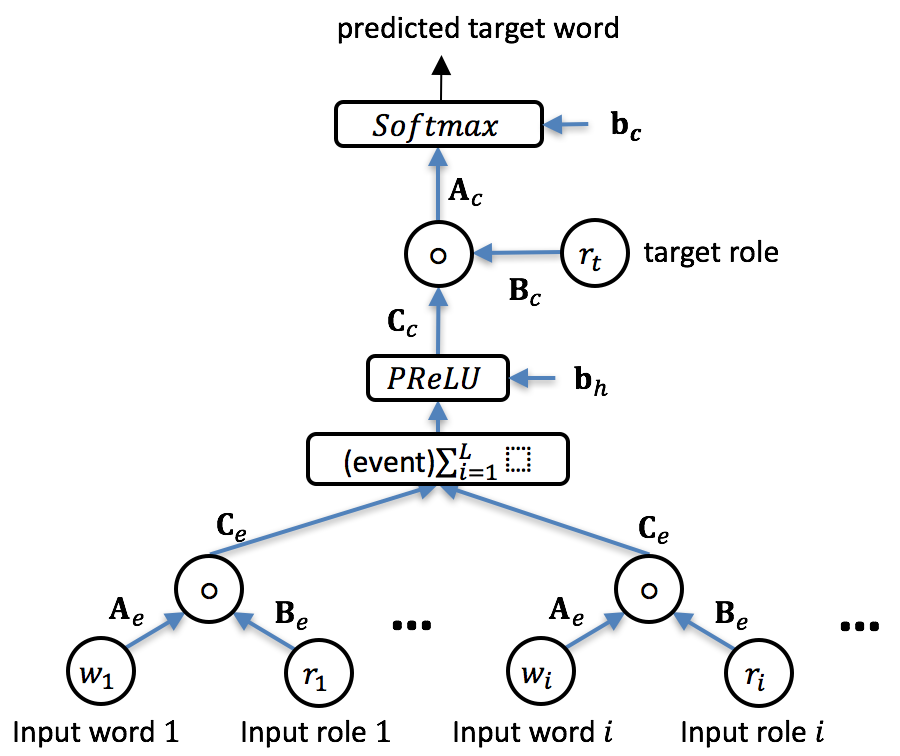
\includegraphics[width=0.65\textwidth]{NNRF.png}
\caption{\label{fig:NNRF} Model architecture of non-incremental role filler.}
\end{figure}


\subsection{Non-incremental Role Filler Model} \label{sec:nnrf}
To perform the role-filler prediction, \citet{tilk2016event} proposed the \textit{non-incremental role filler} \textbf{(NNRF)} which is a 2-layer neural network model. As in Figure \ref{fig:NNRF}, from input to output, the model uses event-participant embeddings as input. Parameters are learnt together with the model. The embedding vector of the $l$-th entry in an event can be represented as:
\begin{equation} \label{eq:rbe-nnrf}
\begin{aligned}
    \mathbf{p}_l
        &= (\mathbf{w}_i \mathbf{A}_e \circ \mathbf{r}_j \mathbf{B}_e) \mathbf{C}_e \\
\end{aligned}
\end{equation}
The embedding vectors are composed using sum method into an representation of words except the target word as:
\begin{equation} \label{eq:sum-comp}
\begin{aligned}
    \mathbf{e}
        &= \sum_{l=1}^{L} \mathbf{p}_{l} \\
\end{aligned}
\end{equation}
where $l$ is the index of the participant and $L$ is the number of participants in current event $e$. Then it passes through one non-linearity layer with parametric rectified linear unit \citep{he2015delving} as follow:
\begin{equation} \label{eq:nonlinearity-nnrf}
\begin{aligned}
    \mathbf{h}
        &= PReLU(\mathbf{e} + \mathbf{b}_e) \\
\end{aligned}
\end{equation}
where $\mathbf{b}_e$ is the bias vector of this layer. After that, a softmax regression classifier is used for prediction. The output vector of this classifier is computed as:
\begin{equation} \label{eq:output-nnrf}
\begin{aligned}
    \mathbf{o}
        &= \mathbf{h}\mathbf{W}_c + \mathbf{b}_c \\
\end{aligned}
\end{equation}
where $\mathbf{W}_c\in \mathbb{R}^{d \times |V|}$ is a weight matrix of the target word classifier and $\mathbf{b}_c$ is the corresponding bias. The conditional probability of target word $a_x$ given event $e$ and target role $b_y$ is:
\begin{equation} \label{eq:softmax-nnrf}
\begin{aligned}
    p(a_x | e, b_y)
        &= Softmax(\mathbf{o})_{(x)} \\
        &= \frac{
        exp(\mathbf{o})_{(x)}
        }{
        \sum_{i=1}^{|V|} exp(\mathbf{o})_{(i)} }   \\
\end{aligned}
\end{equation}
where suffix $(x)$ is the $x$-th element of the vector. 

For each target target role, there is a different weight matrix to perform classification. \citet{tilk2016event} applied a factorisation for the classifiers, which is similar to the method for role-specific word embedding. At first weight matrix $\mathbf{W}_c^{(b_y)}$ is defined for each target role $b_y$. Then those matrices $\mathbf{W}_c^{(b_y)}$ are stacked from $b_1$ to $b_{|R|}$. A weight tensor $\mathbf{T}^{(c)} \in \mathbb{R}^{d \times |R| \times |V|}$ is obtained. But this tensor suffer the same dimensionality problem as event-participant embedding tensor. So tensor rank decomposition is applied again on the weight tensor, and extract the corresponding weight matrices for $b_y$ as follow: 
\begin{equation} \label{eq:trd-cls}
\begin{aligned}
    \mathbf{T}_{(y)}^{(c)}
        &= \sum_{m=1}^{k^{(c)}} \mathbf{c}_{m}^{(c)} \otimes \mathbf{b}_{m_{(y)}}^{(c)} \otimes \mathbf{a}_m^{(c)} \\
\end{aligned}
\end{equation}
Similarly, vectors $\mathbf{c}_{m}^{(c)}$ are grouped by row into matrices $\mathbf{C}_c \in \mathbb{R}^{d \times k^{(c)}}$ and $\mathbf{a}_m^{(c)}$ are grouped by column into matrices $\mathbf{A}_c \in \mathbb{R}^{k^{(c)} \times |V|}$. After getting rid of outer product using same transformation as equation \eqref{eq:rbwe}, the weight matrix in equation \eqref{eq:output-nnrf}  can be written as:
\begin{equation} \label{eq:cls}
\begin{aligned}
    \mathbf{W}_c
        &= \mathbf{C}_c \ diag(\mathbf{b}_y) \ \mathbf{A}_c \\
\end{aligned}
\end{equation}
Since there is a vector $\mathbf{b}_y$ representing target role $b_y$, the embedding matrices $\mathbf{B}_c \in \mathbb{R}^{k^{(c)} \times |R|}$ can be defined for target roles. The weight matrices can be further written as:
\begin{equation} \label{eq:cls-temb}
\begin{aligned}
    \mathbf{W}_c
        &= \mathbf{C}_c \ diag(\mathbf{r}_y \mathbf{B}_c) \ \mathbf{A}_c \\
\end{aligned}
\end{equation}


\begin{figure}[t]
\centering
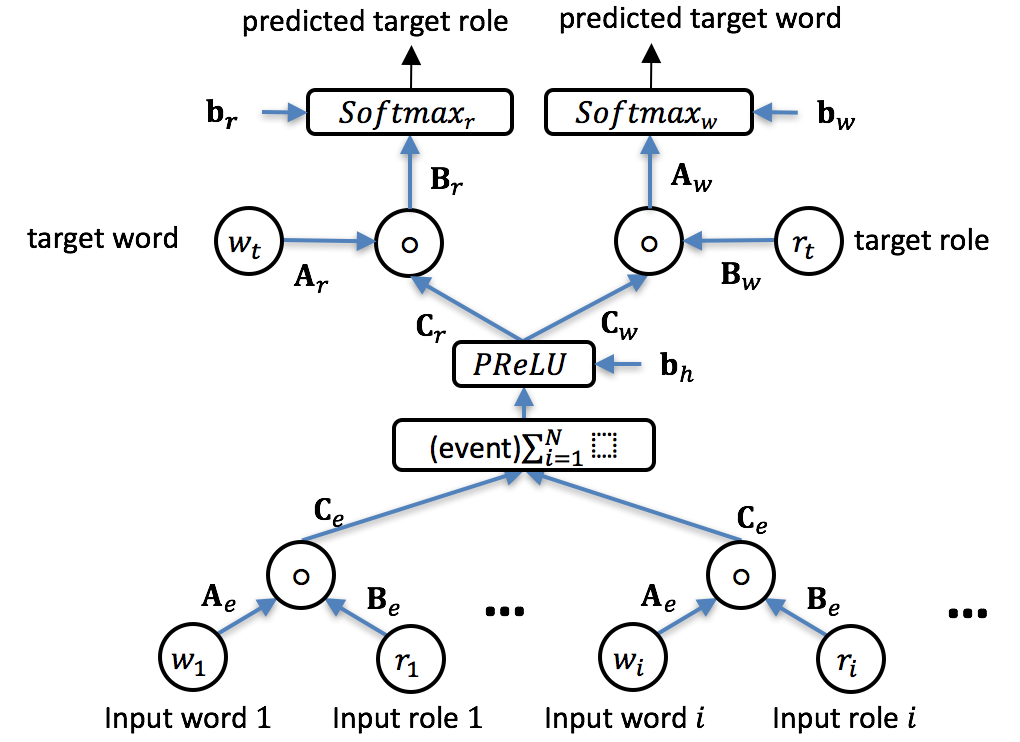
\includegraphics[width=0.7\textwidth]{MTRF.png}
\caption{\label{fig:MTNNRF} Model architecture of multitask version of non-incremental role filler.}
\end{figure}


\subsection{Multitask Learning} \label{sec:mtl}
In addition to role-filler prediction, we also want to perform semantic role prediction. This task can be considered as a regularisation of the objective function of the role-filler prediction task. Using this idea, we design a model named \textbf{multitask role filler (MTRF)} described in Figure \ref{fig:MTNNRF} which differs with \textbf{NNRF} only in the last layer. 

Since we want to obtain the probability distribution of target word or target role, in the last layer a softmax regression classifier is used for each task. The output vectors of these classifiers are computed as:
\begin{equation} \label{eq:output-mt}
\begin{aligned}
    \mathbf{o}_w
        &= \mathbf{e}\mathbf{W}_w + \mathbf{b}_w \\
    \mathbf{o}_r
        &= \mathbf{e}\mathbf{W}_r + \mathbf{b}_r \\
\end{aligned}
\end{equation}
where $\mathbf{W}_w \in \mathbb{R}^{d \times |V|}$ is a weight matrix of the target word classifier,  $\mathbf{W}_r \in \mathbb{R}^{d \times |R|}$ is a weight matrix of the target role classifier and $\mathbf{b}_w$, $\mathbf{b}_r$ are the corresponding biases of the classifier. The conditional probability of target word $a_x$ given event $e$ and target role $b_y$ is:
\begin{equation} \label{eq:softmax-w}
\begin{aligned}
    p(a_x | e, b_y)
        &= Softmax(\mathbf{o}_w)_{(x)} \\
        &= \frac{
        exp(\mathbf{o}_w)_{(x)}
        }{
        \sum_{i=1}^{|V|} exp(\mathbf{o}_w)_{(i)} }   \\
\end{aligned}
\end{equation}
where suffix $(x)$ is the $x$-th element of the vector. And the conditional probability of target role $b_y$ given event $e$ and target word $a_x$ is:
\begin{equation} \label{eq:softmax-r}
\begin{aligned}
    p(b_y | e, a_x)
        &= Softmax(\mathbf{o}_r)_{(y)} \\
        &= \frac{
        exp(\mathbf{o}_r)_{(y)}
        }{
        \sum_{j=1}^{|R|} exp(\mathbf{o}_r)_{(j)} }   \\
\end{aligned}
\end{equation}

For each target role or target word, we apply tensor factorisation again to obtain target role/word specific classifiers. At first we define weight matrix $\mathbf{W}_w$ and weight matrix $\mathbf{W}_r$ for each target word $a_x$ and target role $b_y$. Then we stack $\mathbf{W}_w$ and $\mathbf{W}_r$ from $a_1$ to $a_{|V|}$ and from $b_1$ to $b_{|R|}$. Two weight tensors $\mathbf{T}^{(w)} \in \mathbb{R}^{d \times |R| \times |V|}$ and $\mathbf{T}^{(r)} \in \mathbb{R}^{d \times |V| \times |R|}$ are obtained. But these tensors suffer the same dimensionality problem as event-participant embedding tensor. So we apply tensor rank decomposition again on two weight tensors, and extract the corresponding weight matrices for $a_x$ and $b_y$ as follow: 
\begin{equation} \label{eq:trd-mt-cls}
\begin{aligned}
    \mathbf{T}_{(x)}^{(w)}
        &= \sum_{m=1}^{k^{(w)}} \mathbf{c}_{m}^{(w)} \otimes \mathbf{b}_{m_{(x)}}^{(w)} \otimes \mathbf{a}_m^{(w)} \\
    \mathbf{T}_{(y)}^{(r)}
        &= \sum_{m=1}^{k^{(r)}} \mathbf{c}_{m}^{(r)} \otimes  \mathbf{a}_{m_{(y)}}^{(r)} \otimes \mathbf{b}_m^{(r)} \\
\end{aligned}
\end{equation}
Similarly, we group vectors $\mathbf{c}_{m}^{(w)}$, $\mathbf{c}_{m}^{(r)}$ by row into matrices $\mathbf{C}_w \in \mathbb{R}^{d \times k^{(w)}}$, $\mathbf{C}_r \in \mathbb{R}^{d \times k^{(r)}}$ and group $\mathbf{a}_m^{(w)}$, $\mathbf{b}_m^{(r)}$ by column into matrices $\mathbf{A}_w \in \mathbb{R}^{k^{(w)} \times |V|}$, $\mathbf{B}_r \in \mathbb{R}^{k^{(r)} \times |R|}$. After getting rid of outer product using same transformation as equation \eqref{eq:rbwe}, two weight matrices in equation \eqref{eq:output-nnrf}  can be written as: 
\begin{equation} \label{eq:cls-mt}
\begin{aligned}
    \mathbf{W}_w
        &= \mathbf{C}_w \ diag(\mathbf{b}_y) \ \mathbf{A}_w \\
    \mathbf{W}_r
        &= \mathbf{C}_r \ diag(\mathbf{a}_x) \ \mathbf{B}_r \\
\end{aligned}
\end{equation}
where $diag(\mathbf{v})$ is a diagonal matrix with vector $\mathbf{v}$ on its diagonal. Since there is a vector $\mathbf{b}_y$ representing target role $b_y$ and there is a vector $\mathbf{a}_x$ representing target word $a_x$. Now we can define the embedding matrices $\mathbf{B}_w \in \mathbb{R}^{k^{(w)} \times |R|}$, $\mathbf{A}_r \in \mathbb{R}^{k^{(r)} \times |V|}$ for target roles and target words. The weight matrices can be further written as: 
\begin{equation} \label{eq:cls-mt-temb}
\begin{aligned}
    \mathbf{W}_w
        &= \mathbf{C}_w \ diag(\mathbf{r}_y \mathbf{B}_w) \ \mathbf{A}_w \\
    \mathbf{W}_r
        &= \mathbf{C}_r \ diag(\mathbf{w}_x \mathbf{A}_r) \ \mathbf{B}_r \\
\end{aligned}
\end{equation}


\subsection{Model Comparison} \label{sec:comp_mtrf}
In order to show whether the event similarity problem is solved, we perform a model comparison between NNRF and MTRF. Two models are implemented with the same number of hyper-parameters, except MTRF has additional parameters in the target role classifier. We trained and validated both models on the RW-eng corpus (see Section \ref{sec:corpus}). 

The data set is provided by \citet{grefenstette2015concrete} (see Section \ref{sec:eventsim}). Each row in the data set contains a participant ID, two events, a human evaluation score of their similarity from $1$ to $7$ and a HIGH/LOW tag indicating the similarity group of the entry. An example entry is:
\begin{equation} \label{eg:event-sim}
    participant1, (table, draw, eye), (table, attract, eye), 7, \text{HIGH}
\end{equation}
Naturally we can consider the subject $table$ has a ARG0 semantic role and the object $eye$ has a ARG1 semantic role in the event.

The models are evaluated in two experiments. In the first experiment, for each entry which has a HIGH tag and the highest score (i.e. $7$) in the data set, we extract two events and construct a foil event for the second event. For example entry \eqref{eg:event-sim}, we have:
\begin{equation}
    (table, draw, eye), (table, draw, eye), (eye, attract, table)
\end{equation}
This subset is named as \textbf{foil event similarity (FSM)} data set. We extract the event embedding vector defined in equation  \eqref{eq:sum-comp} from two models. We then compute two similarities: similarity of the first event and the second event; similarity of the first event and the foil event. Generally the larger of the difference between these two similarities we obtain, the better model we have. The similarity score of two events is computed as cosine similarity of two event embedding vectors. For each model, the means of these two similarities are computed across FSM. The results are in Table \ref{tab:foil-mtrf}. MTRF has a lower mean similarity between based event and foil event. Moreover, it has a higher difference between two similarities.

The second experiment is event similarity task \citep{grefenstette2015concrete}. We extract the event embedding vector for the first and second event. The similarity score of two events is computed as cosine similarity as well. Then we compute Spearman's rho correlation coefficient between model scores and human judgement scores. The result in every epoch is reported as a line chart in Figure \ref{fig:GS-NNRF-MTRF}. The correlation score keeps stable after $20$ epochs. MTRF has a higher score than NNRF at almost every epoch. Thus MTRF is better correlated with human performance. This indicates that with the additional semantic role prediction task, MTRF learns a better embedding of events. 


\begin{figure}[t]
\centering
\includegraphics[width=0.9\textwidth]{GS-NNRF-MTRF.png}
\caption{\label{fig:GS-NNRF-MTRF} Event similarity evaluation by training epoch of NNRF and MTRF. $x$-axis is the number of training epochs. $y$-axis is the Spearman's rho between model scores andhuman judgements. }
\end{figure}


\begin{table}[t]
\centering
\begin{tabular}{l|lll}
    \textbf{Model}  &   $cos$(Event 1, Event 2)   &    $cos$(Event 1, Foil Event)    &  Difference  \\ \hline
    \textbf{NNRF}   &   78  &   64  &   14  \\
    \textbf{MTRF}   &   68  &   52  &   \textbf{16}  \\
\end{tabular}
\caption{\label{tab:foil-mtrf} Similar event similarity versus foil event similarity. }
\end{table}
% * <asayeed@mbl.ca> 2017-11-13T22:52:35.875Z:
% 
% Did I miss how many items there were in this data set? Can we get an idea of the significance of this difference? (I realize that this is not always easy to calculate, but at least the data set size and some sort of variances may be useful here.)
% 
% ^.



\newpage
\section{Bag-of-Event-Participant Model} \label{sec:bop}


\begin{figure}[t]
\centering
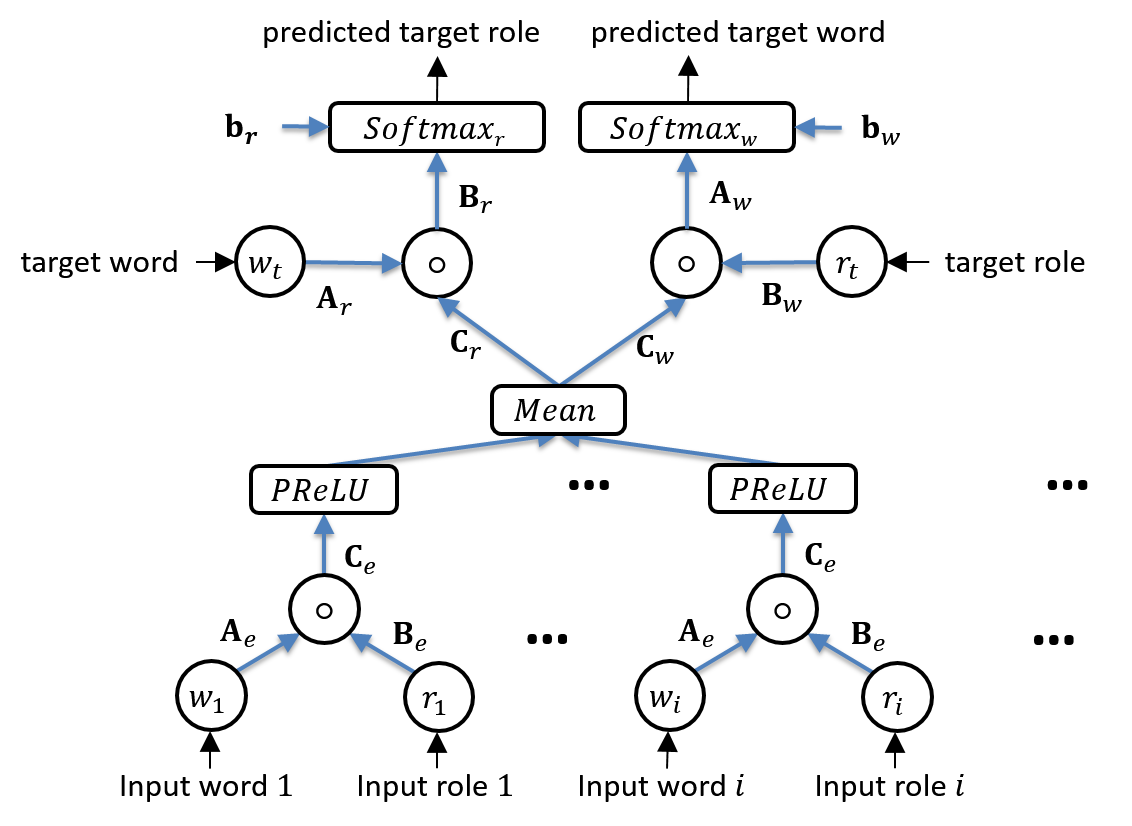
\includegraphics[width=0.8\textwidth]{BOP.png}
\caption{\label{fig:BOP} Model architecture of bag-of-predicates/participants.}
\end{figure}


\subsection{Composition Method for Event Embedding} \label{sec:composition}
In the NNRF model, embedding vectors of event participants are sum up together to represent the whole event. Nonetheless, this is only a simple method to composite event participants. Each participant has the same weight in the event. Additionally, means of parameters can shift in a large range the after the sum operation. How can we improve this? We need an exploration of composition methods. 

We separate all possible methods into two groups. The first group is \textbf{non-parametric methods} which have no extra parameters like addition, multiplication and concatenation of event participant vectors. Another group is \textbf{parametric methods} which need more parameters like recursive unit \citep{socher2013recursive}, recurrent unit \citet{mikolov2010recurrent}, or long-short-term-memory recurrent unit \citep{hochreiter1997LSTM}. So the NNRF is classified as non-parametric composition method. 

The second model proposed by \citet{tilk2016event}, \textit{incremental model}, is a parametric method. A recurrent unit is added to express participant order not only within event but also across different events. Moreover, a binary indicator $b$ is used to detect the event boundaries. $b$ equals to $1$ if the target word belongs to current event, otherwise $0$. So the event embedding vector is: 
\begin{equation} \label{eq:incremental}
\begin{aligned}
    \mathbf{e} 
        &= \mathbf{p} + \mathbf{h_{t-1}}\mathbf{W}_h + b\mathbf{v}, 
\end{aligned}
\end{equation}
where $\mathbf{v}$ is the parameter vector of event boundary. $\mathbf{h_{t-1}}$ is the hidden vector of last time step in the recurrent unit. $\mathbf{W}_h$ is the parameter matrix of recurrent unit. 

\subsection{Mean Composition Method} \label{sec:mean-composition}
In this work, we focus on non-parametric methods in the condition that participant order is not provided and leave the other for future exploration. Multiplication is an effective composition method for distributional memory models. Unfortunately, during optimisation of neural network models, multiplication often results in extreme values which will lead to overflow or underflow. Concatenation is widely used in language modelling. But the concatenated feature cannot be used directly. An extra feature extractor on top of the concatenation is needed, which turns it into a parametric method. 
% * <asayeed@mbl.ca> 2017-11-13T22:54:15.219Z:
% 
% "distributed semantic models" you mean...you're not referring to SDDM here right?
% 
% ^ <xhong@coli.uni-saarland.de> 2017-11-16T13:13:34.064Z:
% 
% Sorry, it is a typo. It is changed to 'distributional memory models'. 
%
% ^ <asayeed@mbl.ca> 2017-11-16T21:57:26.535Z:
% 
% But multiplication *isn't* an effective composition model for DMs due to the sparsity and the tendency to make everything 0.  The whole problem is that no one's been able to make a purely multiplicative model scale, right?
%
% ^.


We propose the \textbf{mean} composition method which computes the mean of all the vectors of event participants to represent the event as one vector. Computing the mean can be considered as normalisation of participant representations within the event boundary, which can prevent possible overflow/underflow of weights of the hidden vector. 

Since it is a non-parametric method, we also want to add a weight before the mean composition. Instead of using a fully-connected layer, we apply the PReLU to each embedding vector of participants to obtain the hidden vector: 
\begin{equation} \label{eq:nonlinearity-bop}
\begin{aligned}
    \mathbf{h}_l
        &= PReLU_l(\mathbf{p}_l) \\
\end{aligned}
\end{equation}
So the parameters inside PReLU can also act as weights of each participant. Using the mean method, the embedding vectors are composed as:
\begin{equation} \label{eq:mean-comp-bop}
\begin{aligned}
    \mathbf{e}
        &= \frac{1}{L} \sum_{l=1}^{L} \mathbf{h}_{l} \\
\end{aligned}
\end{equation}
whehe $\frac{1}{L}$ is used to compute the empirical mean of the hidden vector. This model is named as \textbf{bag-of-predicates/participants (BOP)} described in Figure \ref{fig:BOP}. 


\begin{figure}[t]
\centering
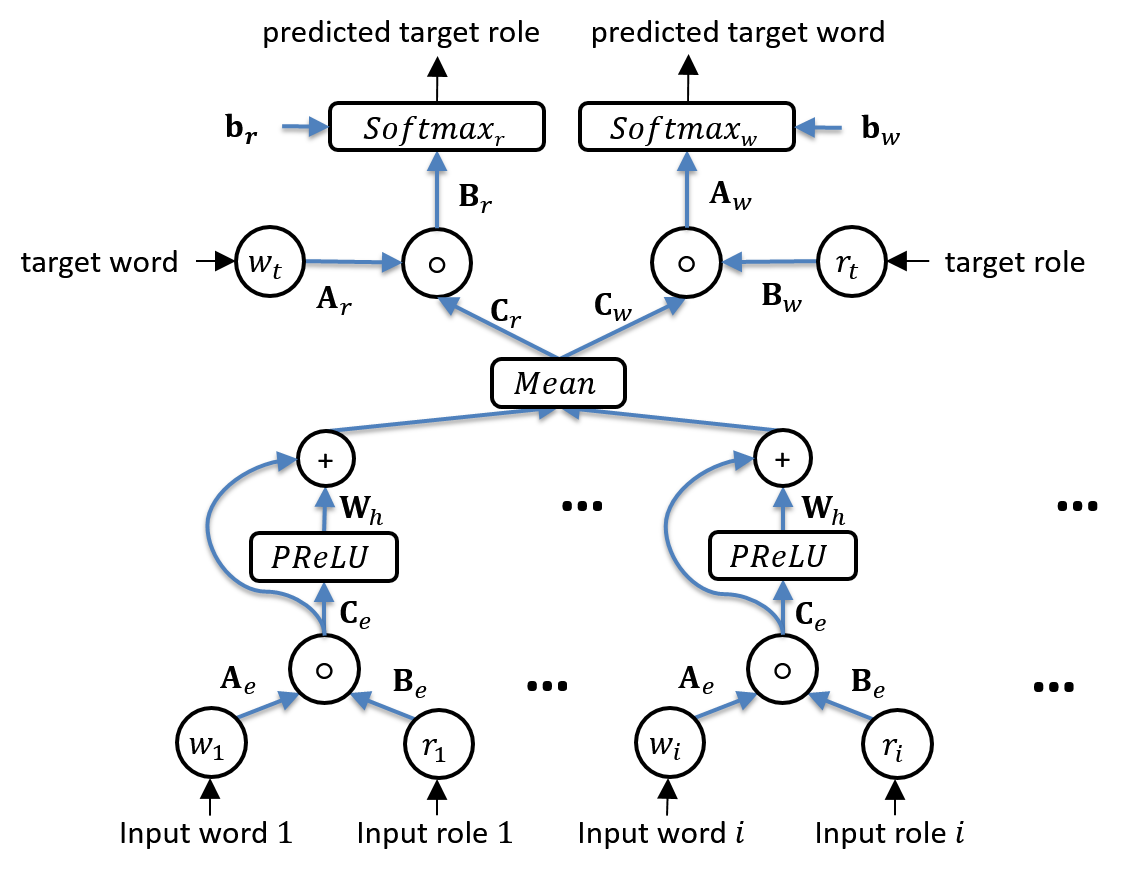
\includegraphics[width=0.8\textwidth]{BOPRes.png}
\caption{\label{fig:BOPRes} Model architecture of bag-of-predicates/participants with residual learning.}
\end{figure}

% * <asayeed@mbl.ca> 2017-11-13T22:55:19.201Z:
% 
% Would be worth it to maybe highlight somehow visually the differences between these models? As in the most salient feature that distinguishes them from each other/NNRF?
% 
% ^ <xhong@coli.uni-saarland.de> 2017-11-16T13:14:37.312Z:
% 
% I updated with newest figures.  Do you mean I should write them in the text?
% 
% ^ <asayeed@mbl.ca> 2017-11-16T21:58:28.689Z:
% 
% Might be worth pointing out what your highlights mean.  Clarity never hurt.
%
% ^.

\subsection{Residual Learning} \label{sec:residual}
All models presented above contain two factored tensors. It has been shown that training model with factored tensors is difficult \citep{sutskever2011generating, kiros2014multimodal}. Due to the fact that each tensor element is represented as a product of three parameters, gradient explosion or vanishing problem happens more likely during the training. To tackle the gradient explosion or vanishing problem in deep neural networks, \citet{he2016deep} proposed the \textit{deep residual learning} framework. They have the observation that in a way of constructing a deep model from a shallow model, one needs to add additional layers which are identity mapping over other layers copied from the shallow model. As a result, we can force the layers to fit a residual mapping. Formally, a residual block containing two hidden layers using $PReLU$ activation function can be written as: 
\begin{equation} \label{eq:res-block}
\begin{aligned}
    \mathbf{h}^{(1)}
        &= PReLU(\mathbf{x}\mathbf{W}^{(1)}) \\
    \mathbf{h}^{(2)}
        &= PReLU(\mathbf{h}^{(1)}\mathbf{W}^{(2)} + \mathbf{x}) \\
\end{aligned}
\end{equation}
Inspiring by this idea, we employ residual learning in our BOP model. For the event-participant embedding in equation \eqref{eq:rbe-nnrf}, there are two product operators, the Hadamard product and the dot product. We want to construct the residual block here to separate weight flow between two product operators. So we rewrite the event-participant embedding vector as: 
\begin{equation} \label{eq:rbe-bopres}
\begin{aligned}
    \mathbf{p}_l
        &= (\mathbf{w}_i \mathbf{A}_e \circ \mathbf{r}_j \mathbf{B}_e) \mathbf{C}_e \\
        &= \mathbf{r}_l \mathbf{C}_e \\
\end{aligned}
\end{equation}
where $\mathbf{r}_l$, the composition of word embedding and semantic role label embedding, is treated as the residual. The original weight of the event-participant embedding goes into non-linear layer as equation \eqref{eq:nonlinearity-bop} and then dot products the weight matrix $\mathbf{W}_h$, but the weight of the residual goes into the event embedding directly as:
\begin{equation} \label{eq:hidden-bopres}
\begin{aligned}
    & \mathbf{h}_l^{(1)}
        = PReLU_l(\mathbf{r}_l \mathbf{C}_e) \\
    & \mathbf{h}_{l}
        = \mathbf{h}_{l}^{(1)}\mathbf{W}_h + \mathbf{r}_l \\
\end{aligned}
\end{equation}
Then the model perform the mean composition as  equation \eqref{eq:mean-comp-bop}. Since we only have one non-linearity layer in BOP, so the second non-linearity layer in residual block is removed. This model is named as \textbf{bag-of-predicates/participants with residual learning (BOP Res)} described in Figure \ref{fig:BOPRes}. 


\subsection{Model Comparison} \label{sec:comp-bop}



\newpage
\section{Experiments}  \label{sec:exp}
\subsection{Corpus and Prepossessing} \label{sec:corpus}
We use Rollenwechsel-English (RW-eng) corpus, a large-scale labelled semantic corpus with a head word of each argument using PropBank style role labels \citep{SayeedEtAl2015}. With head words of arguments, we have a direct access to the event participants without modifiers. This helps us to learn embeddings of generalised event knowledge. 

The corpus, extracted from the ukWaC corpus \citep{ferraresi2008introducing} and BNC \citep{british2007british}, contains about 78 million sentences over 2.3 million documents. Among those sentences, there are approximately 210 million event predicates and 710 million event participants. They divided the corpus into 3500 segments with approximately same number of documents. The sentences are labelled using SENNA, a syntactic agnostic semantic role labeller with competitive performance. The head words are extracted with four heuristics: \texttt{MALT}, \texttt{MALT-SPAN}, \texttt{LINEAR} and \texttt{FAILED}. 

One sample event in the corpus is here:
\definecolor{bg}{rgb}{0.95, 0.95, 0.95}
\begin{minted}
[frame=lines,
framesep=2mm,
baselinestretch=1.2,
bgcolor=bg,
fontsize=\footnotesize,
linenos]{xml}
<text id="ukwac:http://www.exeterviews.co.uk/exeter-shopping2.php" />
<s>
<predicate>
  <governor>release/vbg/13</governor>
  <dependencies>
    <dep algorithm="MALT" source="the/DT/3 large/JJ/4
    stone/NNS/5" text="the large stone"
    type="A0">stone/nns/5</dep>
    <dep algorithm="FAILED" source="which/WDT/6" text="which"
    type="R-A0">which/wdt/6</dep>
    <dep source="release/VBG/13"
    text="release" type="V">release/vbg/13</dep>
    <dep algorithm="MALT_SPAN" source="their/PRP$/14 heat/NN/15"
    text="their heat" type="A1">heat/nn/15</dep>
    <dep algorithm="LINEAR" source="at/IN/16 night/NN/17"
    text="at night" type="AM-TMP">night/nn/17</dep>
    <dep algorithm="MALT" source="to/TO/18 ensure/VB/19 the/DT/20
    grape/NNS/21 achieve/VBP/22 maximum/JJ/23 ripeness/NN/24"
    text="to ensure the grape achieve maximum ripeness"
    type="AM-PNC">achieve/vbp/22</dep>
  </dependencies>
</predicate>
\end{minted}
where event is arranged in XML format.  

We choose the first 3472 segments as training data, the next 14 segments as testing data and the last 14 segments as validation data. The word vocabulary for event predicates and participants is constructed with following steps: 
\begin{enumerate}
  \item  go through the training data, for each event, find out the entries denoting the event predicate and all event participants. 
  \item  filter out every entry with FAILED tag in $algorithm$ attribute; only accept entry with POS tag starting with $n$, $v$, $j$, $r$; only accept entry with English characters and punctuation like $'$, $-$; 
  \item  extract the lowercase form of the head word from each entry.
  \item  lemmatized each word using WordNet lemmatizer in NLTK. 
  \item  compute the frequency of each unique lemma. 
  \item  generate the vocabulary from the top 50000 most frequent words. 
\end{enumerate}


\subsection{Model Implementation} \label{sec:implementation}
We implement the models with Keras 2.0.5 \citep{chollet2015keras}. And then we deploy each model on high performance computer with one 48 cores Intel Xeon E7 CPU and one Nvidia Geforce Titan X GPU as neural network accelerator. 



\newpage
\section{Evaluation}  \label{sec:evaluation}
\subsection{Participant and Predicate Prediction}  \label{sec:wordprediction}


\begin{table}[t]
\centering
\begin{tabular}{l|l|l||l|l|l|l||l}
Dataset &   TypeDM  &   SDDM    &   NNRF    &   MTRF    &   BOP &   BOP Res     &   BOP Res*    \\ \hline
P07     &   53      &   51      &   48      &   48      &   52  &   \textbf{54} &   51          \\
MSTNN   &   32      &   24      &   39      &   39      &   42  &   \textbf{42} &   42          \\
F-Loc   &   23      &   19      &   51      &   48      &   44  &   45          &   44          \\
F-Inst  &   36      &   19      &   51      &   50      &   49  &   \textbf{51} &   50          \\
GDS-all &   53      &   40      &   62      &   61      &   60  &   61          &   61          \\
\end{tabular}
\caption{\label{tab:widgets} Experiment result of models on human thematic fit judgement correlation task.}
\end{table}


\subsection{Semantic Role Prediction}  \label{sec:roleprediction}

\subsection{Human Thematic Fit Judgement Correlation Task}  \label{sec:thematicfit}
To improve the performance of DM on thematic fit task, \citet{greenberg2015improving} employed clustering on candidate role-fillers to construct a better representation for prototypical role-filler. They obtained good performance in less frequent roles like INSTRUMENT and LOCATION. 

\subsection{Word Similarity Correlation Task}  \label{sec:wordsim}


\subsection{Event Similarity Correlation Task}  \label{sec:eventsim}
We use the dataset proporsed by \citet{grefenstette2015concrete}.
We choose the result at the $30$-th epoch as the final result and compare these two systems with previous state-of-the-art models. The result is in Table \ref{tab:GS_mtrf}. 


\begin{table}[t]
\centering
\begin{tabular}{l||lll|ll|l}
\textbf{Model}          &   Add &   Kronecker   &   CBOW    &   NNRF    &   MTRF        &   Human   \\ \hline
\textbf{$\rho$ * 100}   &   10  &   26          &   13      &   32 (34) &   \textbf{35} &   62      \\
\end{tabular}
\caption{\label{tab:GS_mtrf} Event similarity evaluation comparing to previous models. $p\text{-value} < 0.05$ for all results. }
\end{table}
% * <asayeed@mbl.ca> 2017-11-13T22:59:17.281Z:
% 
% The meaning of this needs quite a bit more in-context explanation I think.  But I suppose that's why it's at the end here :)
% 
% ^.



\section{Related Works}



\section{Conclusion} 
\subsection{Summary of This Paper} 



\subsection{Future Works}



\newpage


\bibliographystyle{acl_natbib}
\bibliography{mtrf}



\end{document}